
%----------------------------------------------------------------------------------------------------------------------
\begin{frame}{Testing}
\begin{itemize}[noitemsep,label=\textbullet,topsep=2pt,parsep=2pt,partopsep=2pt]
\item Objective: To test and assess 
\item Academic models for simplicity in explanations
\item Module specific models
\item Real life part: ``Enclosure''
	\begin{itemize}[noitemsep,label=\textbullet,topsep=2pt,parsep=2pt,partopsep=2pt]
	\item Outer casing, two flaps with holes for screw fitments. 
	\item Slots for interfaces to external environment. 
	\item Embossed name, chute, slots for guiding wires in place. 
	\end{itemize}
\vspace{-.25cm}
%\includegraphics[scale=0.65]{../Common/images/idealization.jpg}
\includegraphics[width=0.45\linewidth]{../Common/images/SheetMetal_Medium_Enclosure_OriginalPart}
\end{itemize}

%Notes: 

\end{frame}


%----------------------------------------------------------------------------------------------------------------------

\begin{frame}{Benchmarking Midsurface}
\def\myfigenlosurebenchmarkcolumnwidth{0.45}
\begin{figure}[!h]
\centering     %%% not \center
\subfloat[Input Part]{\label{fig:results:originalenclosurepart}\includegraphics[width=\myfigenlosurebenchmarkcolumnwidth\linewidth,valign=t]{../Common/images/SheetMetal_Medium_Enclosure_OriginalPart}} \quad
\subfloat[Commercial Application]{\label{fig:results:midsurfbyinventorexnclosure}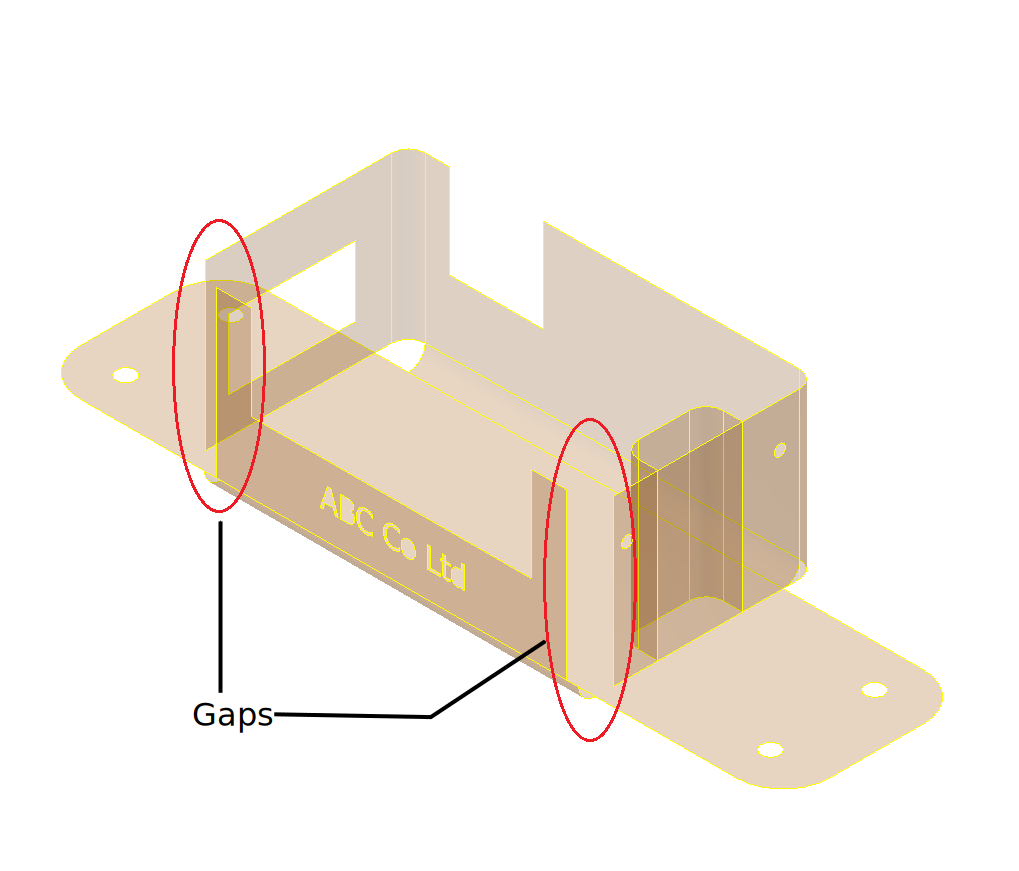
\includegraphics[width=\myfigenlosurebenchmarkcolumnwidth\linewidth,valign=t]{../Common/images/SheetMetal_Medium_Enclosure_InventorMidsurfwithErrors}}
\end{figure}
Quite a few failures are seen, such as disconnected patches, missing midsurface patches etc. 
\end{frame}


%----------------------------------------------------------------------------------------------------------------------
\begin{frame}{Simplification}
\begin{itemize}[noitemsep,label=\textbullet,topsep=2pt,parsep=2pt,partopsep=2pt]
\item Removes unwanted features to compute the ``gross shape''. 
\item Caches tool-bodies of non-suppressible negative features to be used for piercing after midsurface computation. 
\end{itemize}
\def\myfigenlosuredefeaturecolumnwidth{0.95}
\def\myfigenlosuredefeatureTreecolumnwidth{0.75}
\begin{tabular}[h]{@{} p{0.18\linewidth}  p{0.38\linewidth} p{0.1\linewidth} p{0.2\linewidth}@{}}
\toprule
 & Model & Tree & Explanation \\
 \midrule
 
Original/Input &
\raisebox{-0.8\height}{\includegraphics[width=\myfigenlosuredefeaturecolumnwidth\linewidth]{..//Common/images/SheetMetal_Medium_Enclosure_OriginalPart}} &
\raisebox{-0.8\height}{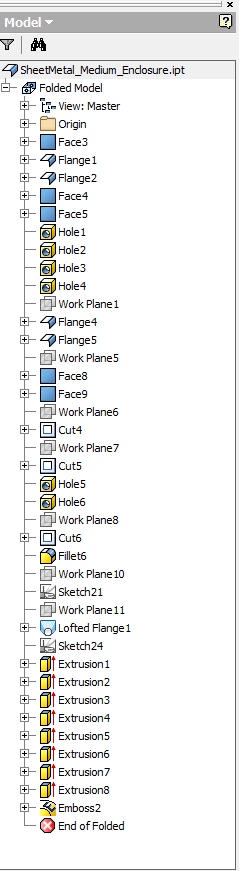
\includegraphics[width=\myfigenlosuredefeatureTreecolumnwidth\linewidth]{..//Common/images/SheetMetal_Medium_Enclosure_OriginalTree}} &

Input with Sheet Metal features.\\

\bottomrule
\end{tabular}

\end{frame}

%----------------------------------------------------------------------------------------------------------------------
\begin{frame}{Phase I}

\def\myfigenlosuredefeaturecolumnwidth{0.95}
\def\myfigenlosuredefeatureTreecolumnwidth{0.75}
\begin{tabular}[h]{@{} p{0.18\linewidth}  p{0.38\linewidth} p{0.1\linewidth} p{0.2\linewidth}@{}}
\toprule
 & Model & Tree & Explanation \\
 \midrule
 
Phase I Selections &
\raisebox{-0.8\height}{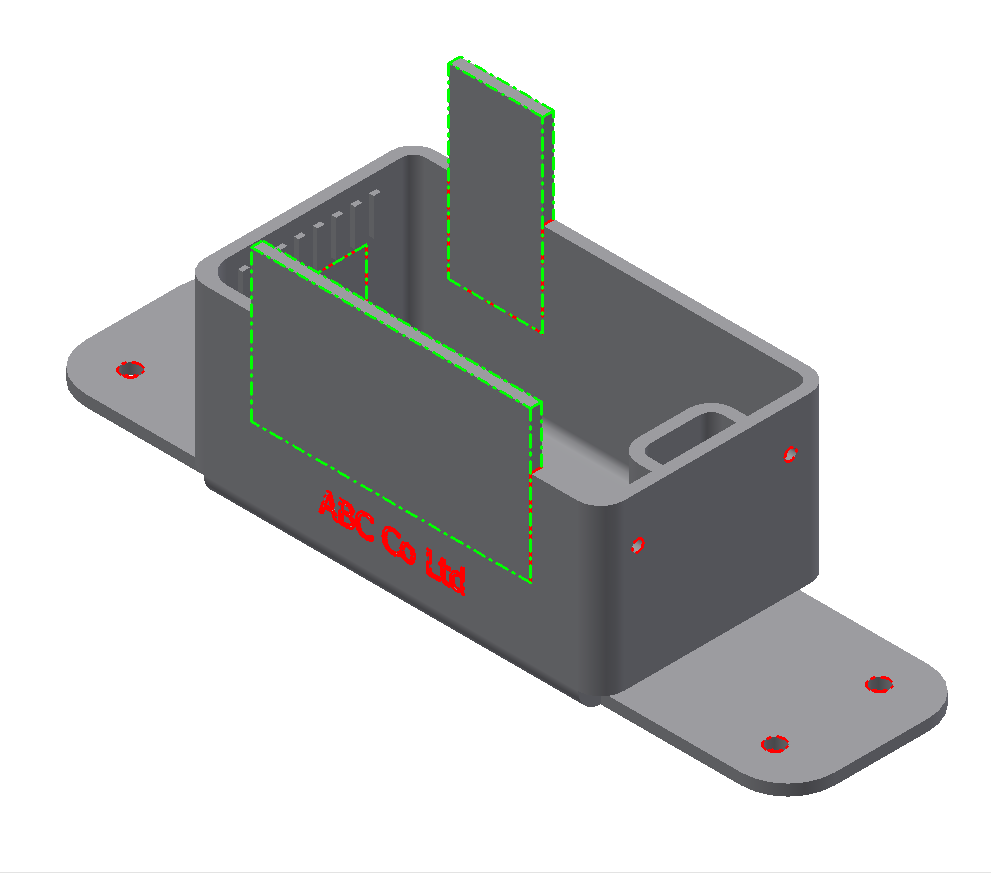
\includegraphics[width=\myfigenlosuredefeaturecolumnwidth\linewidth]{..//Common/images/SheetMetal_Medium_Enclosure_PhaseISelections}} &
\raisebox{-0.8\height}{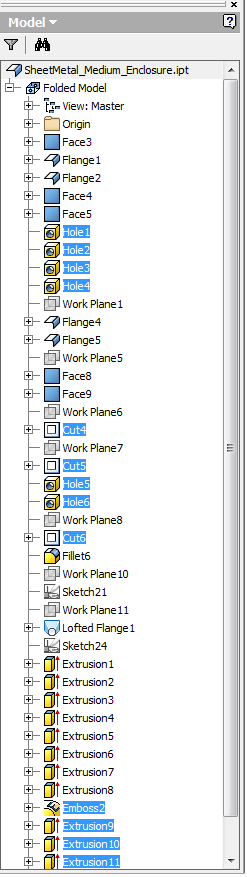
\includegraphics[width=\myfigenlosuredefeatureTreecolumnwidth\linewidth]{..//Common/images/SheetMetal_Medium_Enclosure_PhaseISelectionsTree}} &

Small holes, embossing is chosen based on Sheet Metal feature taxonomy rules (shown red). The green selections are the dormant feature bodies cached.\\

\bottomrule
\end{tabular}

\end{frame}

%----------------------------------------------------------------------------------------------------------------------
\begin{frame}{Phase II}

\def\myfigenlosuredefeaturecolumnwidth{0.95}
\def\myfigenlosuredefeatureTreecolumnwidth{0.75}
\begin{tabular}[h]{@{} p{0.18\linewidth}  p{0.38\linewidth} p{0.1\linewidth} p{0.2\linewidth}@{}}
\toprule
 & Model & Tree & Explanation \\
 \midrule
 
Phase II  Selections&
\raisebox{-0.8\height}{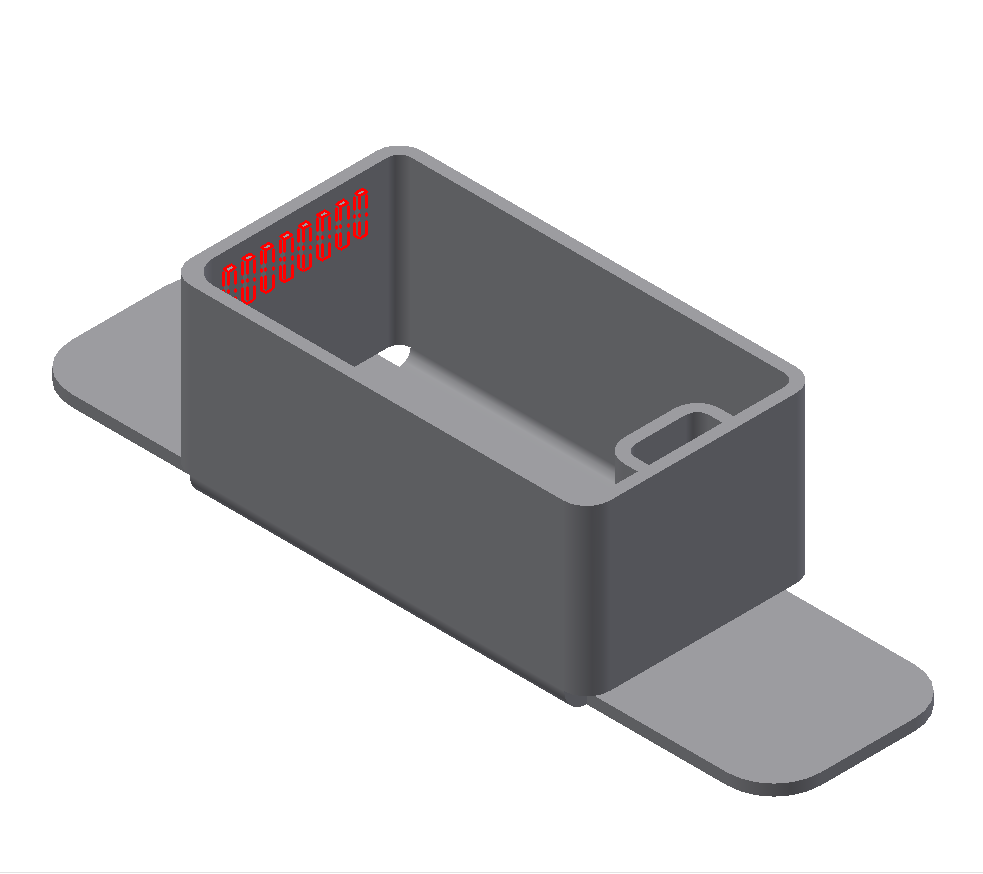
\includegraphics[width=\myfigenlosuredefeaturecolumnwidth\linewidth]{..//Common/images/SheetMetal_Medium_Enclosure_PhaseIISelections}} &
\raisebox{-0.8\height}{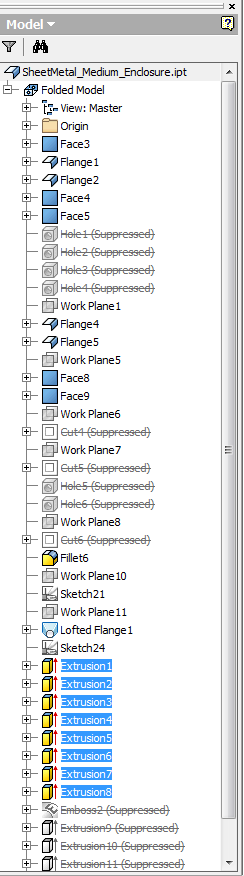
\includegraphics[width=\myfigenlosuredefeatureTreecolumnwidth\linewidth]{..//Common/images/SheetMetal_Medium_Enclosure_PhaseIISelectionsTree}} &

Remnant features got selected in the second phase. \\

\bottomrule
\end{tabular}

\end{frame}

%----------------------------------------------------------------------------------------------------------------------
\begin{frame}{Output}

\def\myfigenlosuredefeaturecolumnwidth{0.95}
\def\myfigenlosuredefeatureTreecolumnwidth{0.75}
\begin{tabular}[h]{@{} p{0.18\linewidth}  p{0.38\linewidth} p{0.1\linewidth} p{0.2\linewidth}@{}}
\toprule
 & Model & Tree & Explanation \\
 \midrule
 
Defeatured&
\raisebox{-0.8\height}{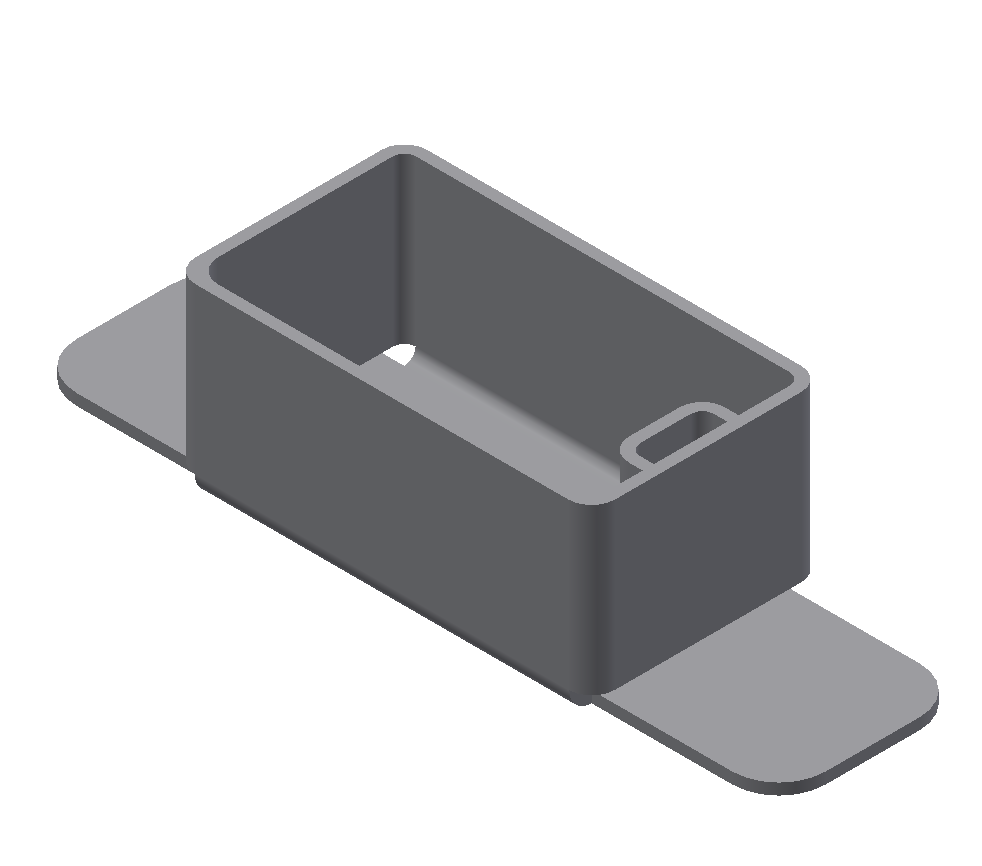
\includegraphics[width=\myfigenlosuredefeaturecolumnwidth\linewidth]{..//Common/images/SheetMetal_Medium_Enclosure_DefeaturedPart}} &
\raisebox{-0.8\height}{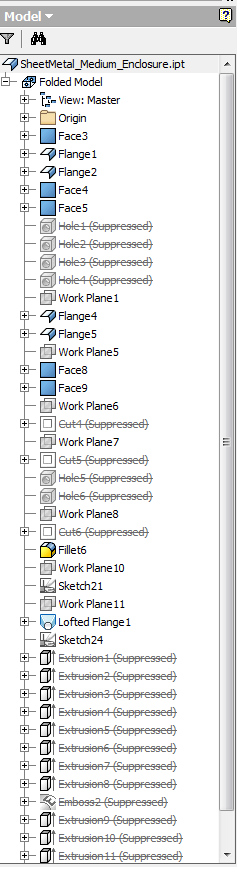
\includegraphics[width=\myfigenlosuredefeatureTreecolumnwidth\linewidth]{..//Common/images/SheetMetal_Medium_Enclosure_DefeaturedTree}} &

Most of the unnecessary features are removed and now it retains all the necessary features adequately ``representing''  the gross shape. \\

\bottomrule
\end{tabular}

\end{frame}

%----------------------------------------------------------------------------------------------------------------------
\begin{frame}{Effectiveness}

Effectiveness with 5\% threshold, based on the criterion defined is:


\begin{tabular}[h]{@{} p{0.22\linewidth} p{0.18\linewidth} p{0.21\linewidth} p{0.2\linewidth} @{}}\toprule
\textbf{Qty} & \textbf{Input} & \textbf{Phase I} & \textbf{Output}\\  \midrule
Faces  & 259 & 104 & 64\\
Suppressed  &  &13 & 8\\
\bottomrule
\end{tabular}

\bigskip

$pR = (1 - \frac{64}{259}) \times 100 = 75.29\%$

\bigskip

Even after huge reduction in the number of faces (75\%), the overall shape of the enclosure is retained fine.

\end{frame}

%----------------------------------------------------------------------------------------------------------------------
\begin{frame}{Abstraction}

\begin{itemize}[noitemsep,label=\textbullet,topsep=2pt,parsep=2pt,partopsep=2pt]
\item To transform sheet metal feature tree into  $\mathcal{ABLE}$ feature (Extrude, Revolve, Sweep, Loft) tree. 
\item Effectiveness is in the faithful reproduction of the part, without any feature or shape loss.
\end{itemize}


\def\myfigenlosuredefeaturecolumnwidth{0.95}
\def\myfigenlosureabelcolumnwidth{0.98}
\begin{tabular}[h]{@{} p{0.12\linewidth}  p{0.38\linewidth} p{0.15\linewidth} p{0.2\linewidth}@{}} \midrule

Abstracted Output &
\raisebox{-0.8\height}{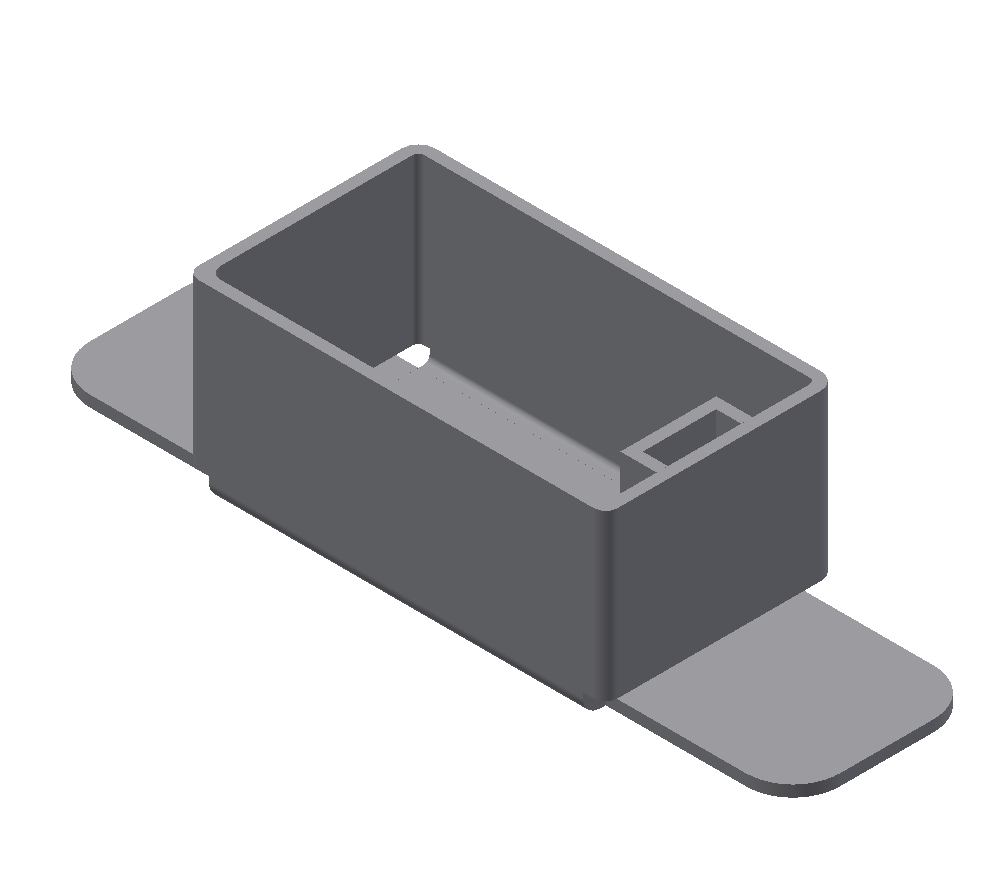
\includegraphics[width=\myfigenlosuredefeaturecolumnwidth\linewidth]{..//Common/images/SheetMetal_Medium_Enclosure_abel_part}} &
\raisebox{-0.8\height}{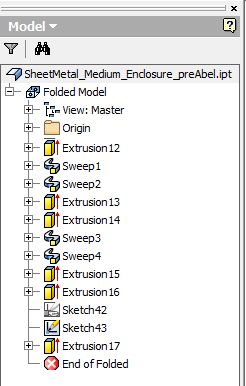
\includegraphics[width=\myfigenlosureabelcolumnwidth\linewidth]{..//Common/images/SheetMetal_Medium_Enclosure_abel_tree}} &

All Sheet Metal features are abstracted/converted to basic primitive features such as Extrude, Sweep etc.\\

\bottomrule
\end{tabular}

\end{frame}

%----------------------------------------------------------------------------------------------------------------------
\begin{frame}{Decomposition}

\begin{itemize}[noitemsep,label=\textbullet,topsep=2pt,parsep=2pt,partopsep=2pt]
\item Decomposition is a manual process. 
\item Feature partitioning:  Internal as well as external booleans  are changed to the ``New Body''
\item Concave edge partitioning:  Overlapping volumes are split at concave edges.
\end{itemize}


\def\myfigenlosuredefeaturecolumnwidth{0.95}
\def\myfigenlosureabelcolumnwidth{0.98}
\begin{tabular}[h]{@{} p{0.15\linewidth}  p{0.38\linewidth} p{0.15\linewidth} p{0.2\linewidth}@{}} \midrule

Decomposed Output &
\raisebox{-0.8\height}{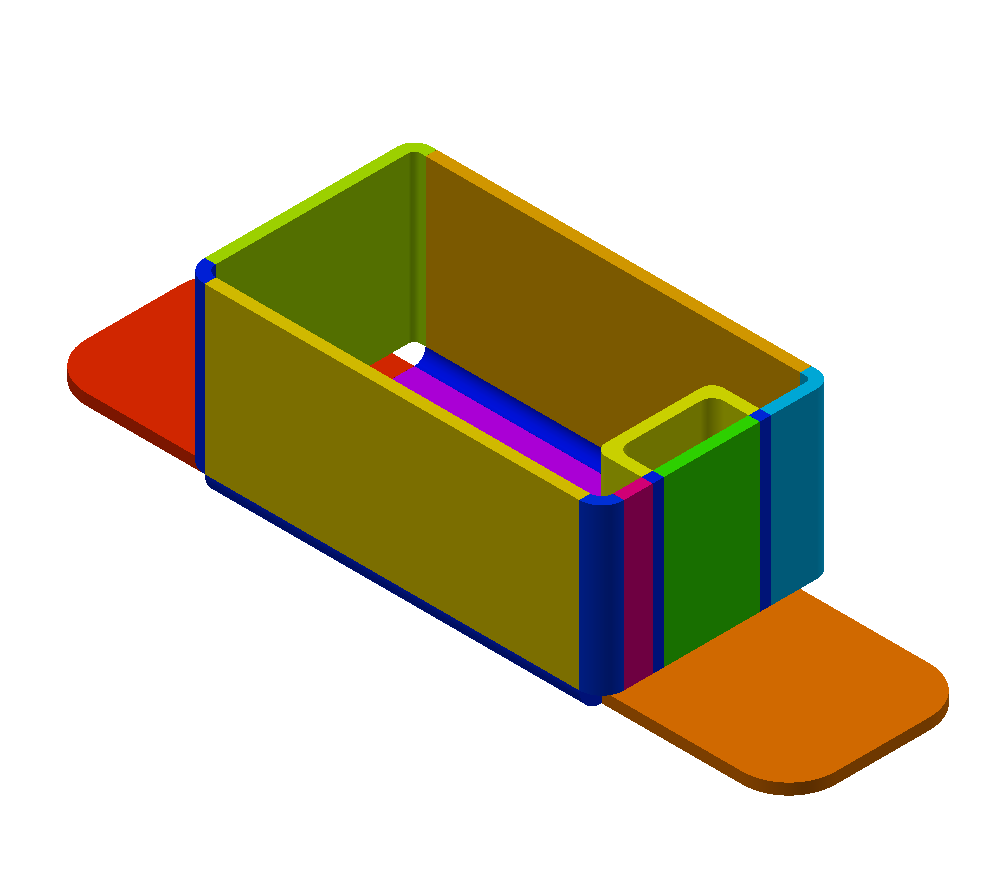
\includegraphics[width=\myfigenlosuredefeaturecolumnwidth\linewidth]{..//Common/images/SheetMetal_Medium_Enclosure_decomp_part}} &
\raisebox{-0.8\height}{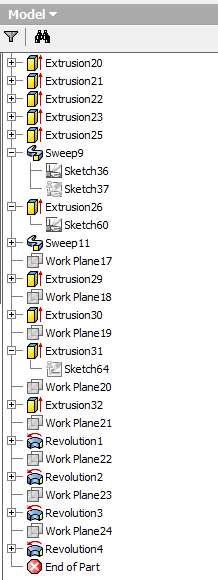
\includegraphics[width=\myfigenlosureabelcolumnwidth\linewidth]{..//Common/images/SheetMetal_Medium_Enclosure_decomp_tree}} &

List of sub-voumnes/cells with a primitive/$\mathcal{ABLE}$ owner feature assigned.\\

\bottomrule
\end{tabular}

\end{frame}

%----------------------------------------------------------------------------------------------------------------------
\begin{frame}{Computation}

\begin{itemize}[noitemsep,label=\textbullet,topsep=2pt,parsep=2pt,partopsep=2pt]
\item Midsurface patches and connections are computed 
\item Dormant bodies cached during defeaturing module are brought back to pierce into this midsurface, so as to generate the pending cuts.
\end{itemize}

\vspace{-.5cm}

\def\myfigenlosurebenchmarkcolumnwidth{0.45}
\begin{figure}[!h]
\centering     %%% not \center
\subfloat[Original Part]{\label{fig:results:originalenclosurepart}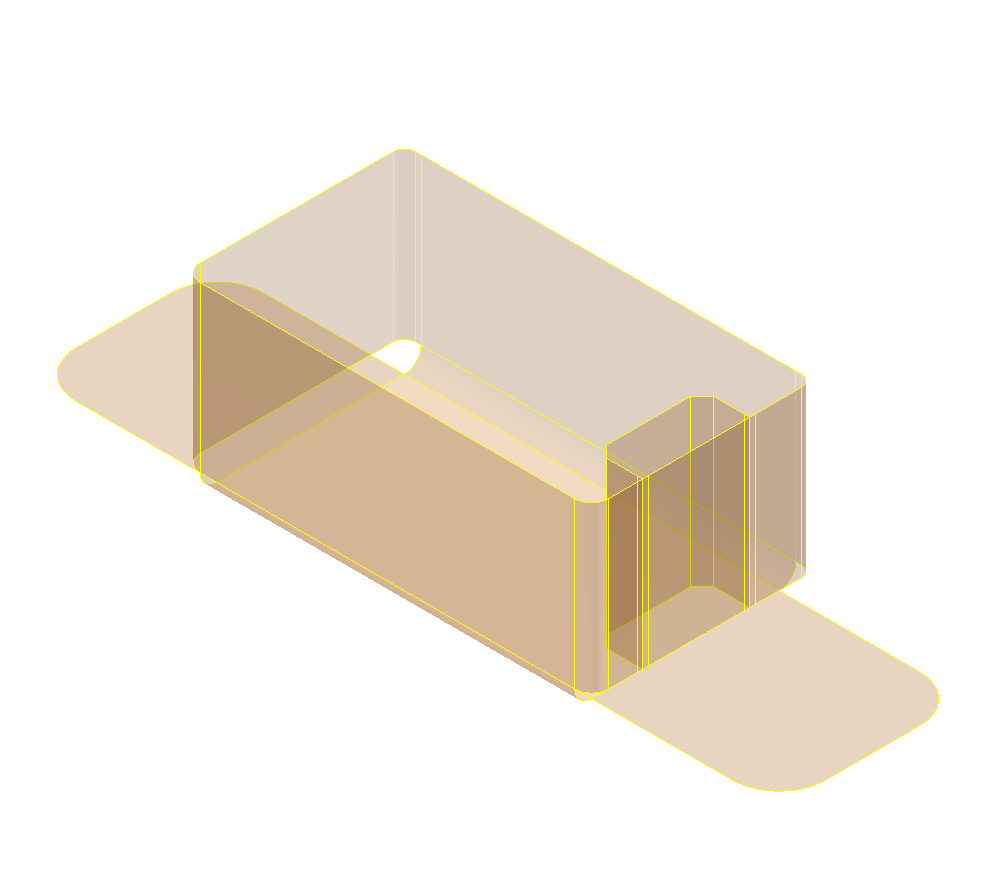
\includegraphics[width=\myfigenlosurebenchmarkcolumnwidth\linewidth,valign=t]{../Common/images/SheetMetal_Medium_Enclosure_midsurf_part}} \quad
\subfloat[Dormant Piercing]{\label{fig:results:midsurfbyinventorexnclosure}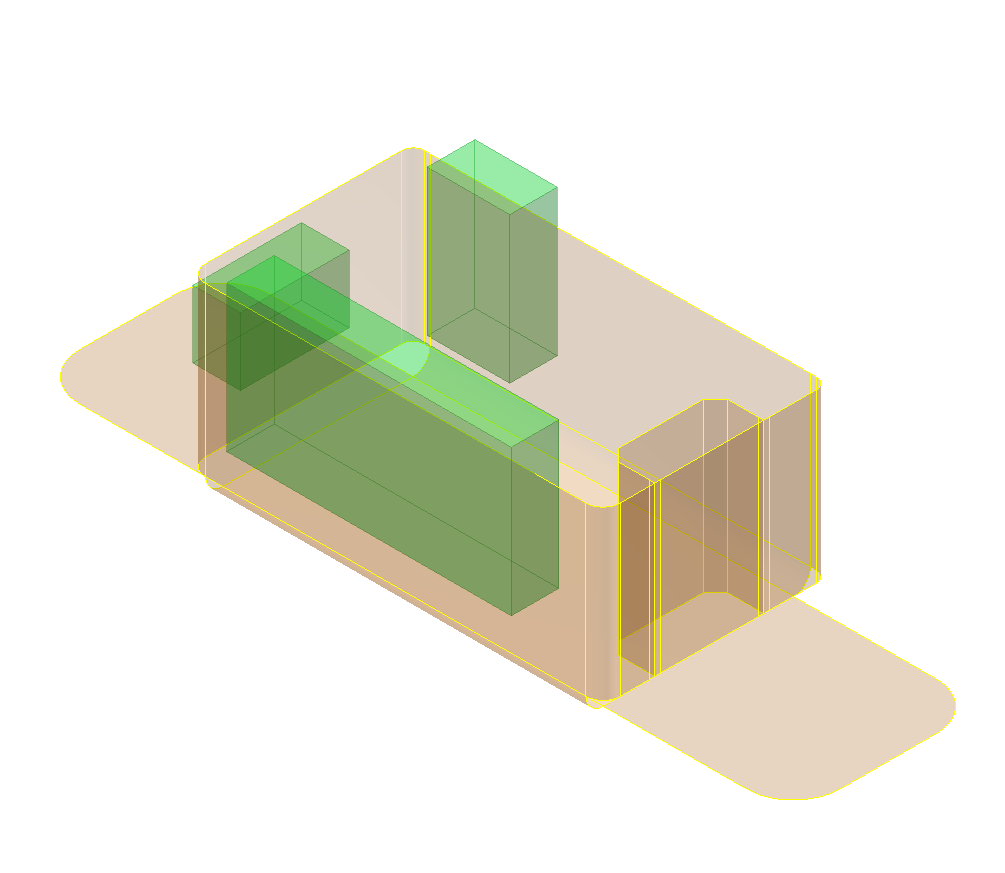
\includegraphics[width=\myfigenlosurebenchmarkcolumnwidth\linewidth,valign=t]{../Common/images/SheetMetal_Medium_Enclosure_dormant_part}}
\end{figure}

\end{frame}

%----------------------------------------------------------------------------------------------------------------------
\begin{frame}{Final Midsurface}

\def\myfigenlosurebenchmarkcolumnwidth{0.45}
\begin{figure}[!h]
\centering     %%% not \center
\subfloat[Original Part]{\label{fig:results:originalenclosurepart}\includegraphics[width=\myfigenlosurebenchmarkcolumnwidth\linewidth,valign=t]{../Common/images/SheetMetal_Medium_Enclosure_OriginalPart}} \qquad
\subfloat[This Research]{\label{fig:results:mymidsurfenclosure}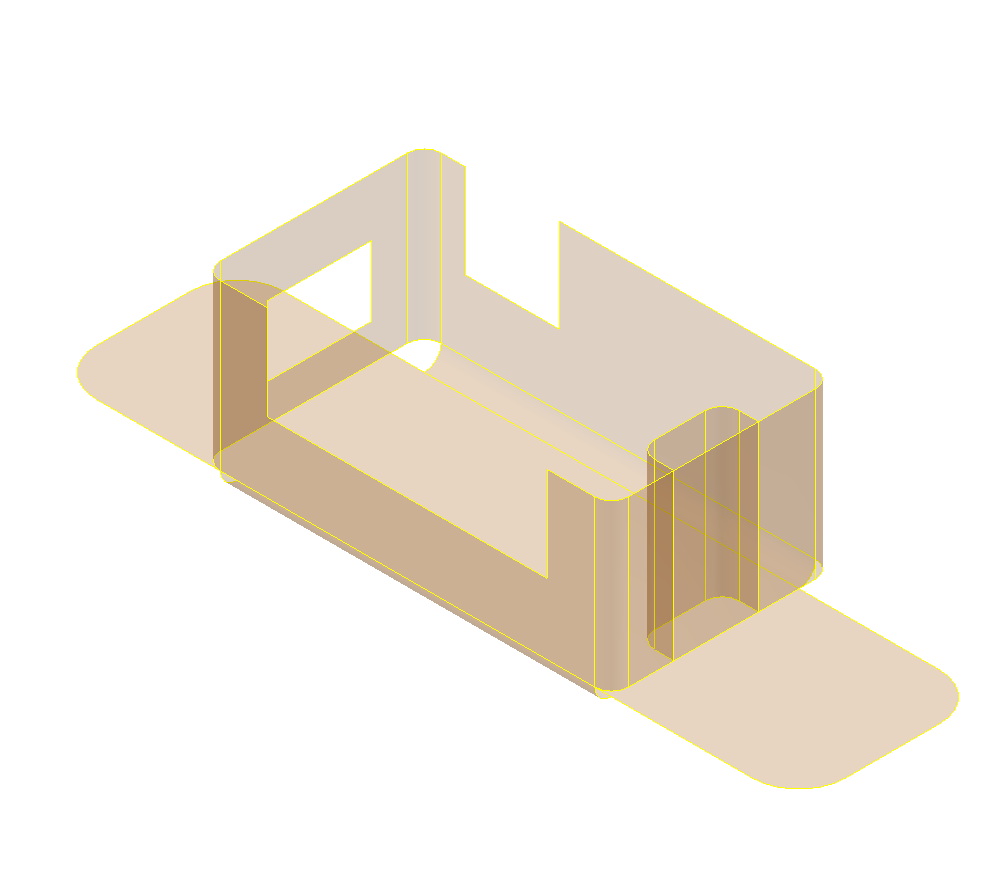
\includegraphics[width=\myfigenlosurebenchmarkcolumnwidth\linewidth,valign=t]{../Common/images/SheetMetal_Medium_Enclosure_final_midsurf_part}}
\end{figure}


\end{frame}

